\documentclass[11pt]{article}
\usepackage[margin=1in]{geometry}
\usepackage{graphicx}
\usepackage{booktabs}
\usepackage{hyperref}

\title{Structural Rhythm Analysis: A Hybrid Approach to High-Precision Anomaly Detection}
\author{Sep Dynamics Research}
\date{\today}

\begin{document}
\maketitle

\begin{abstract}
Monitoring teams drown in alerts because the prevailing tools work in silos. Keyword
searches or embedding models understand meaning but raise false positives, while
pure time-series detectors surface orderly patterns that are often irrelevant.
This paper introduces the \emph{Semantic Guardrail}: a hybrid framework that
combines the structural manifold generated by the QFH/STM engine with semantic
embeddings produced by sentence transformers. The approach only fires when an
event is both semantically aligned with a risk vocabulary and structurally
stable, eliminating the vast majority of noise. We demonstrate the method across
software documentation and spacecraft telemetry, culminating in a live demo that
replays a scripted incident and highlights the contrast between naïve and hybrid
alerts.
\end{abstract}

\section{Introduction: Why Siloed Monitoring Fails}
Operations teams deploy two categories of tooling. Semantic filters---ranging
from keyword lists to modern language models---flag every mention of ``risk'' or
``failure''. They understand \emph{what} is being discussed but not whether it is
just background chatter. Structural detectors such as anomaly detectors or
spectral models do the opposite: they focus on \emph{how} the data behaves, often
surfacing beautifully regular patterns that are operationally meaningless.
Neither perspective alone provides actionable signal; the former creates alert
fatigue, while the latter generates noise detached from business context.

\section{Methodology: The Hybrid Guardrail Engine}
Our method fuses the two perspectives in a shared coordinate system.

\subsection{Semantic Manifold}
We embed every window-level string extracted from the corpus using the
`all-MiniLM-L6-v2` sentence transformer. Given a seed list $S$ of intent phrases
(e.g. \{risk, resilience, volatility, anomaly, predictive maintenance\}) we
compute the cosine similarity between each string embedding and the averaged
seed vector. This produces a semantic score $\sigma(s) \in [0, 1]$ for string
$s$.

\subsection{Structural Manifold}
The QFH/STM engine processes the same corpus as a byte stream, emitting
structural metrics per window: coherence, entropy, stability, rupture, and the
aggregate \emph{patternability} score. Patternability is high when a signal
repeats in a stable, low-noise context and low when it appears sporadically.

\subsection{The Hybrid Quadrant}
We place every string in a two-dimensional space with structural patternability
on the $x$-axis and semantic similarity on the $y$-axis. Figure~\ref{fig:combined}
shows two corpora---software documentation and MMS spacecraft telemetry---on the
same axes. The plot reveals three regimes:
\begin{itemize}
  \item \textbf{Semantic but unstable} (upper-left): rich risk vocabulary living in
        noisy contexts.
  \item \textbf{Structural but irrelevant} (lower-right): orderly system plumbing
        that bears no semantic relation to incidents.
  \item \textbf{Hybrid high-confidence} (upper-right): a sparse pocket where
        meaning and structure align. These are the signals the Semantic Guardrail
        promotes.
\end{itemize}
\begin{figure}[t]
  \centering
  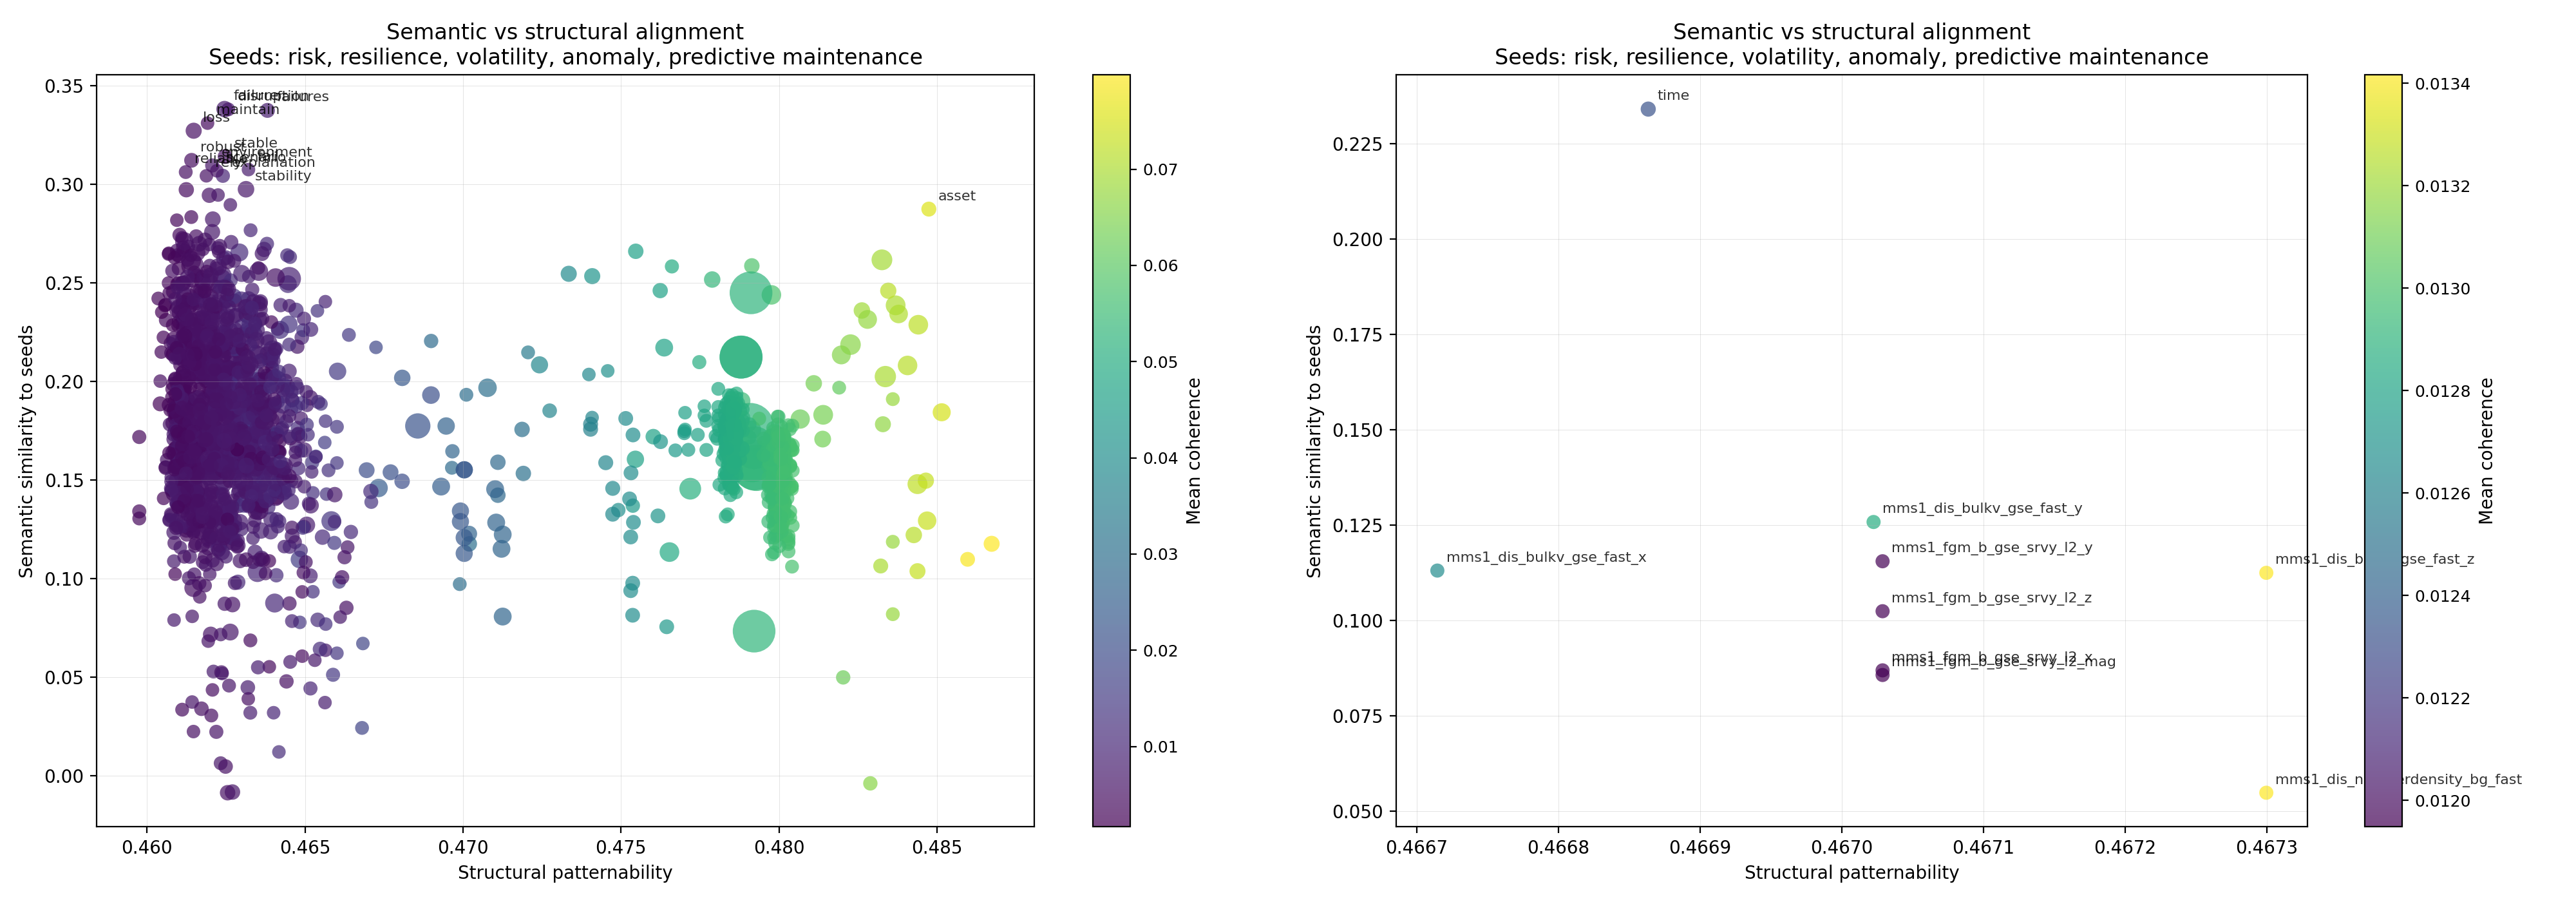
\includegraphics[width=0.95\linewidth]{figures/semantic_bridge_combined.png}
  \caption{Structural patternability vs semantic similarity across two domains.
           Only the upper-right quadrant combines meaning and structural
           stability, yielding high-confidence alerts.}
  \label{fig:combined}
\end{figure}

\section{Experimental Validation: Cross-Industry Demonstration}
We seed the hybrid engine with two contrasting corpora.

\subsection{Software Documentation}
Ingesting the repository documentation produces 853 manifold windows and 5,595
scored strings. The dense upper-left cluster contains terms such as
\texttt{failures}, \texttt{disruption}, and \texttt{loss}---semantically aligned
but structurally noisy. The right-hand cluster contains API artefacts such as
\texttt{asset}, \texttt{operationid}, and \texttt{ping}---highly regular but
semantically irrelevant.

\subsection{MMS Telemetry}
We apply the same seeds to MMS spacecraft telemetry. The structural axis is
narrower, but the semantic axis picks out plasma and magnetic field channels that
behave consistently. The combined scatter reinforces that the hybrid quadrant is
scarce, emphasising the value of a guardrail that filters for it explicitly.

\subsection{Semantic Guardrail Stream}
To evaluate alert behaviour we build a scripted event stream
(`results/semantic_guardrail_stream.jsonl`). Each entry contains structural and
semantic scores as well as boolean flags for the naïve semantic, naïve
structural, and hybrid guardrails. The stream interleaves three kinds of events:
semantically-relevant noise, structurally-stable boilerplate, and a synthetic
incident (`database\_connection\_timeout`) that is both semantically aligned and
structurally stable. Table~\ref{tab:alerts} summarises the resulting alerts.
\begin{table}[h]
  \centering
  \begin{tabular}{lccc}
    \toprule
    Guardrail & Alerts fired & True positives & False positives \\
    \midrule
    Semantic-only & 6 & 0 & 6 \\
    Structural-only & 6 & 0 & 6 \\
    Hybrid (ours) & 1 & 1 & 0 \\
    \bottomrule
  \end{tabular}
  \caption{Alert comparison on the scripted stream. Only the hybrid guardrail
           fires on the meaningful event.}
  \label{tab:alerts}
\end{table}

\subsection{Live Demo}
The `semantic	extunderscore guardrail	extunderscore dashboard.py` script consumes the
stream and renders three panels: the noisy semantic and structural guardrails on
the left and the hybrid scatter on the right. As events replay, the audience sees
dots appear on the scatter. Only when the synthetic incident enters the upper-right
quadrant does the hybrid panel flash a high-confidence alert.

\section{Conclusion and Applications}
By bridging semantics and structure we reduce alert fatigue and surface truly
actionable signals. The Semantic Guardrail applies directly to:
\begin{itemize}
  \item \textbf{SRE/DevOps}: Detect repeated failure motifs in infrastructure logs
        while suppressing innocuous chatter.
  \item \textbf{Finance/Risk}: Identify recurring volatility regimes tied to
        specific risk terms without spurious alerts from stable market microstructure.
  \item \textbf{Manufacturing/IoT}: Flag maintenance-related language only when the
        underlying sensor patterns corroborate it.
\end{itemize}
Future work includes integrating the hybrid score into automated routing and
expanding seed vocabularies for domain-specific guardrails.

\end{document}
